% !TEX root = ../main.tex

\subsection{Results}
With the implementation and analysis out of the way, we can begin to experiment with the echo effect. There is one parameter to adjust: The delay \emph{d}. We have taken a binary approach, starting from Fs and halving the delay each time. The results are shown in \cref{tbl:echo}.
\begin{table}[!hbt]
	\centering
	\begin{tabular}{ccc}
		\toprule
		Units of delay & Time [ms] & Effect \\ 
		\midrule
		44100 & 1000 & Late echo \\ 
		22050 & 500 & Late echo \\ 
		11025 & 250 & Echo \\ 
		5513 & 125 & Echo \\ 
		2757 & 62.5 & Hard to distinguish tracks \\ 
		1379 & 31.3 & Hard to distinguish tracks \\ 
		690 & 15.6 & Impossible to distinguish tracks \\ 
		173 & 3.9 & Impossible to distinguish tracks \\ 
		\bottomrule
	\end{tabular}
	\caption{Effect of different delays for the echo effect, sample rate of \SI{44100}{\hertz}. Sample used is \cite{audiohello}.}
	\label{tbl:echo}
\end{table}
For the last samples, not only is it impossible to distinguish the tracks, the perceived pitch of the vocal track is also changed. For the cases where the delay is around \SI{50}{\milli\second}, we get the effect we wish to dive in to later: Chorus.

For delays larger than around \SI{100}{\milli\second} we get the effect we are looking for. If we increase the delay even further, the echo effect gets more pronounced. For short samples like the vocal hello track used here, the delay gets large enough to completely separate the two tracks. A visualization of the effects for the longer delays is shown in \cref{fig:echohello}.

\begin{table}[!hbt]
	\centering
	\begin{tabular}{cc}
		\toprule
		Relative amplitude & Effect \\ 
		\midrule
		1 & Echo \\ 
		0.5 & Echo \\ 
		0.25 & Echo \\ 
		0.125 & Slight echo \\ 
		0.063 & No echo \\ 
		0.031 & No echo \\ 
		\bottomrule
	\end{tabular}
	\caption{Effect of different amplitudes for the echo effect, sample rate of \SI{44100}{\hertz}. Delay is \SI{125}{\milli\second}. Sample used is \cite{audiohello}.}
	\label{tbl:echoamp}
\end{table}

In \cref{tbl:echoamp}, the effect of changing the amplitude/gain of the echo is investigated, for a fixed delay time, which was previously found to generate an echo. From this table, we see that the amplitude has to be decreased significantly, before we no longer perceive the duplicate signal as an echo of the first, but rather background noise. If we increase the delay for the last two rows, such that it is \SI{1}{\second} instead of \SI{250}{\milli\second}, we are still able to hear the signal, and again begin to hear it as an echo, although quite delayed. Any further decreases in the amplitude results in the signal getting lost in the background and inaudible.

\begin{figure}[!hbt]
	\centering
	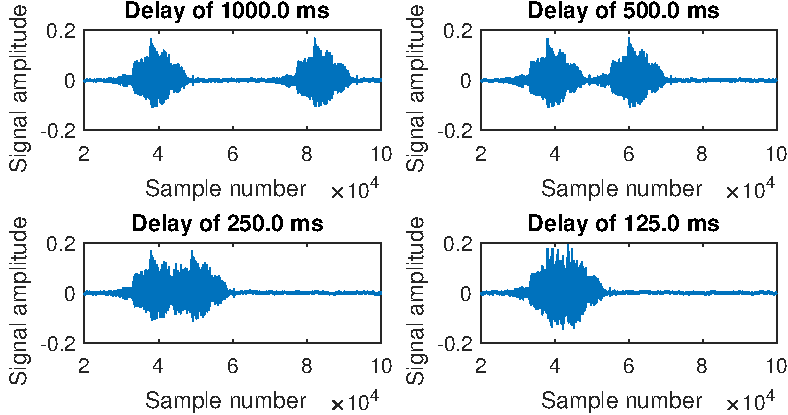
\includegraphics[width=\textwidth]{EchoHello.pdf}
	\caption{Visualization of the echo effect on a track. Sample is from \cite{audiohello}. It can clearly be seen, how the echo joins the main track in time, as the echo delay is reduced.}
	\label{fig:echohello}
\end{figure}

\subsubsection{Monkey Island}
Looking at a complete music sample, instead of a simple "Hello", we turn to the theme from the classic video game Monkey Island. Applying a delay of half a second, with a gain of \num{0.65}, yields the following results in the time and frequency domain.

\begin{figure}[!hbt]
	\centering
	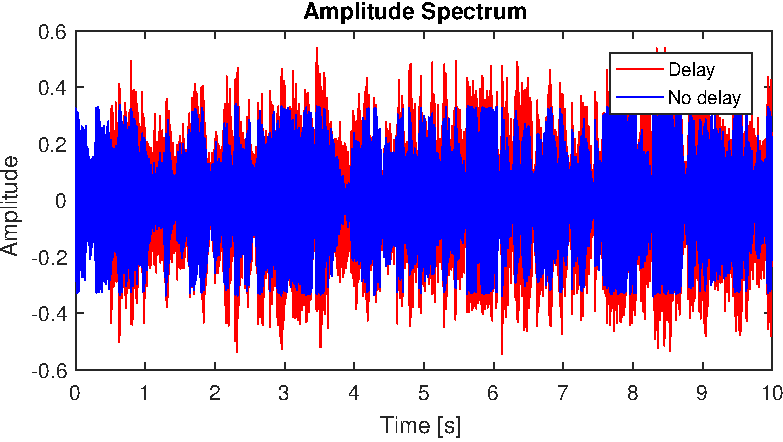
\includegraphics[width=\textwidth]{EchoTime.pdf}
	\caption{Excerpt of the theme from Monkey Island in the time domain, with and without a slight delay to induce an echo effect.}
	\label{fig:echotime}
\end{figure}

\begin{figure}[!hbt]
	\centering
	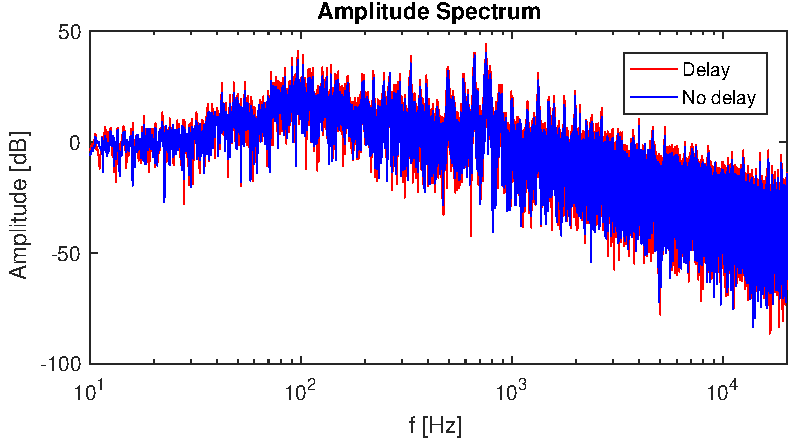
\includegraphics[width=\textwidth]{EchoFreq.pdf}
	\caption{Excerpt of the theme from Monkey Island in the frequency domain, with and without a slight delay to induce an echo effect.}
	\label{fig:echofreq}
\end{figure}

In \cref{fig:echotime}, the results of the echo FIR filter is shown in the time domain. Since the delay is \SI{0.5}{\second}, it is not possible to see a large effect on the signal, except for the added amplitude due to the addition of a duplicate echo signal. Due to the oscillation frequency of the audio signal, it is difficult to shown a zoom, demonstrating the echo/delay effect.

Likewise, in \cref{fig:echofreq}, the results of the FIR filter on the same sample is shown in the frequency domain. Since the FIR filter only changes amplitudes, we would expect the frequency components to be the same, but the amplitudes changed. This is also evident from the figure, where a slight gain can be observed due to the additional signal. Since the DFT does not tell anything about the timing of the signals, we cannot readily see the echo signal from this.
